\documentclass{subfiles}

\begin{document}
    \subaufgabe{}
        Bei der Emission eines Photons durch ein Elektron $e^{-}\stackrel{\gamma}{\longrightarrow}e^-+\gamma$ lässt sich mittels Feynmandiagramm darstellen:
        
        \begin{figure}[H]
            \centering
            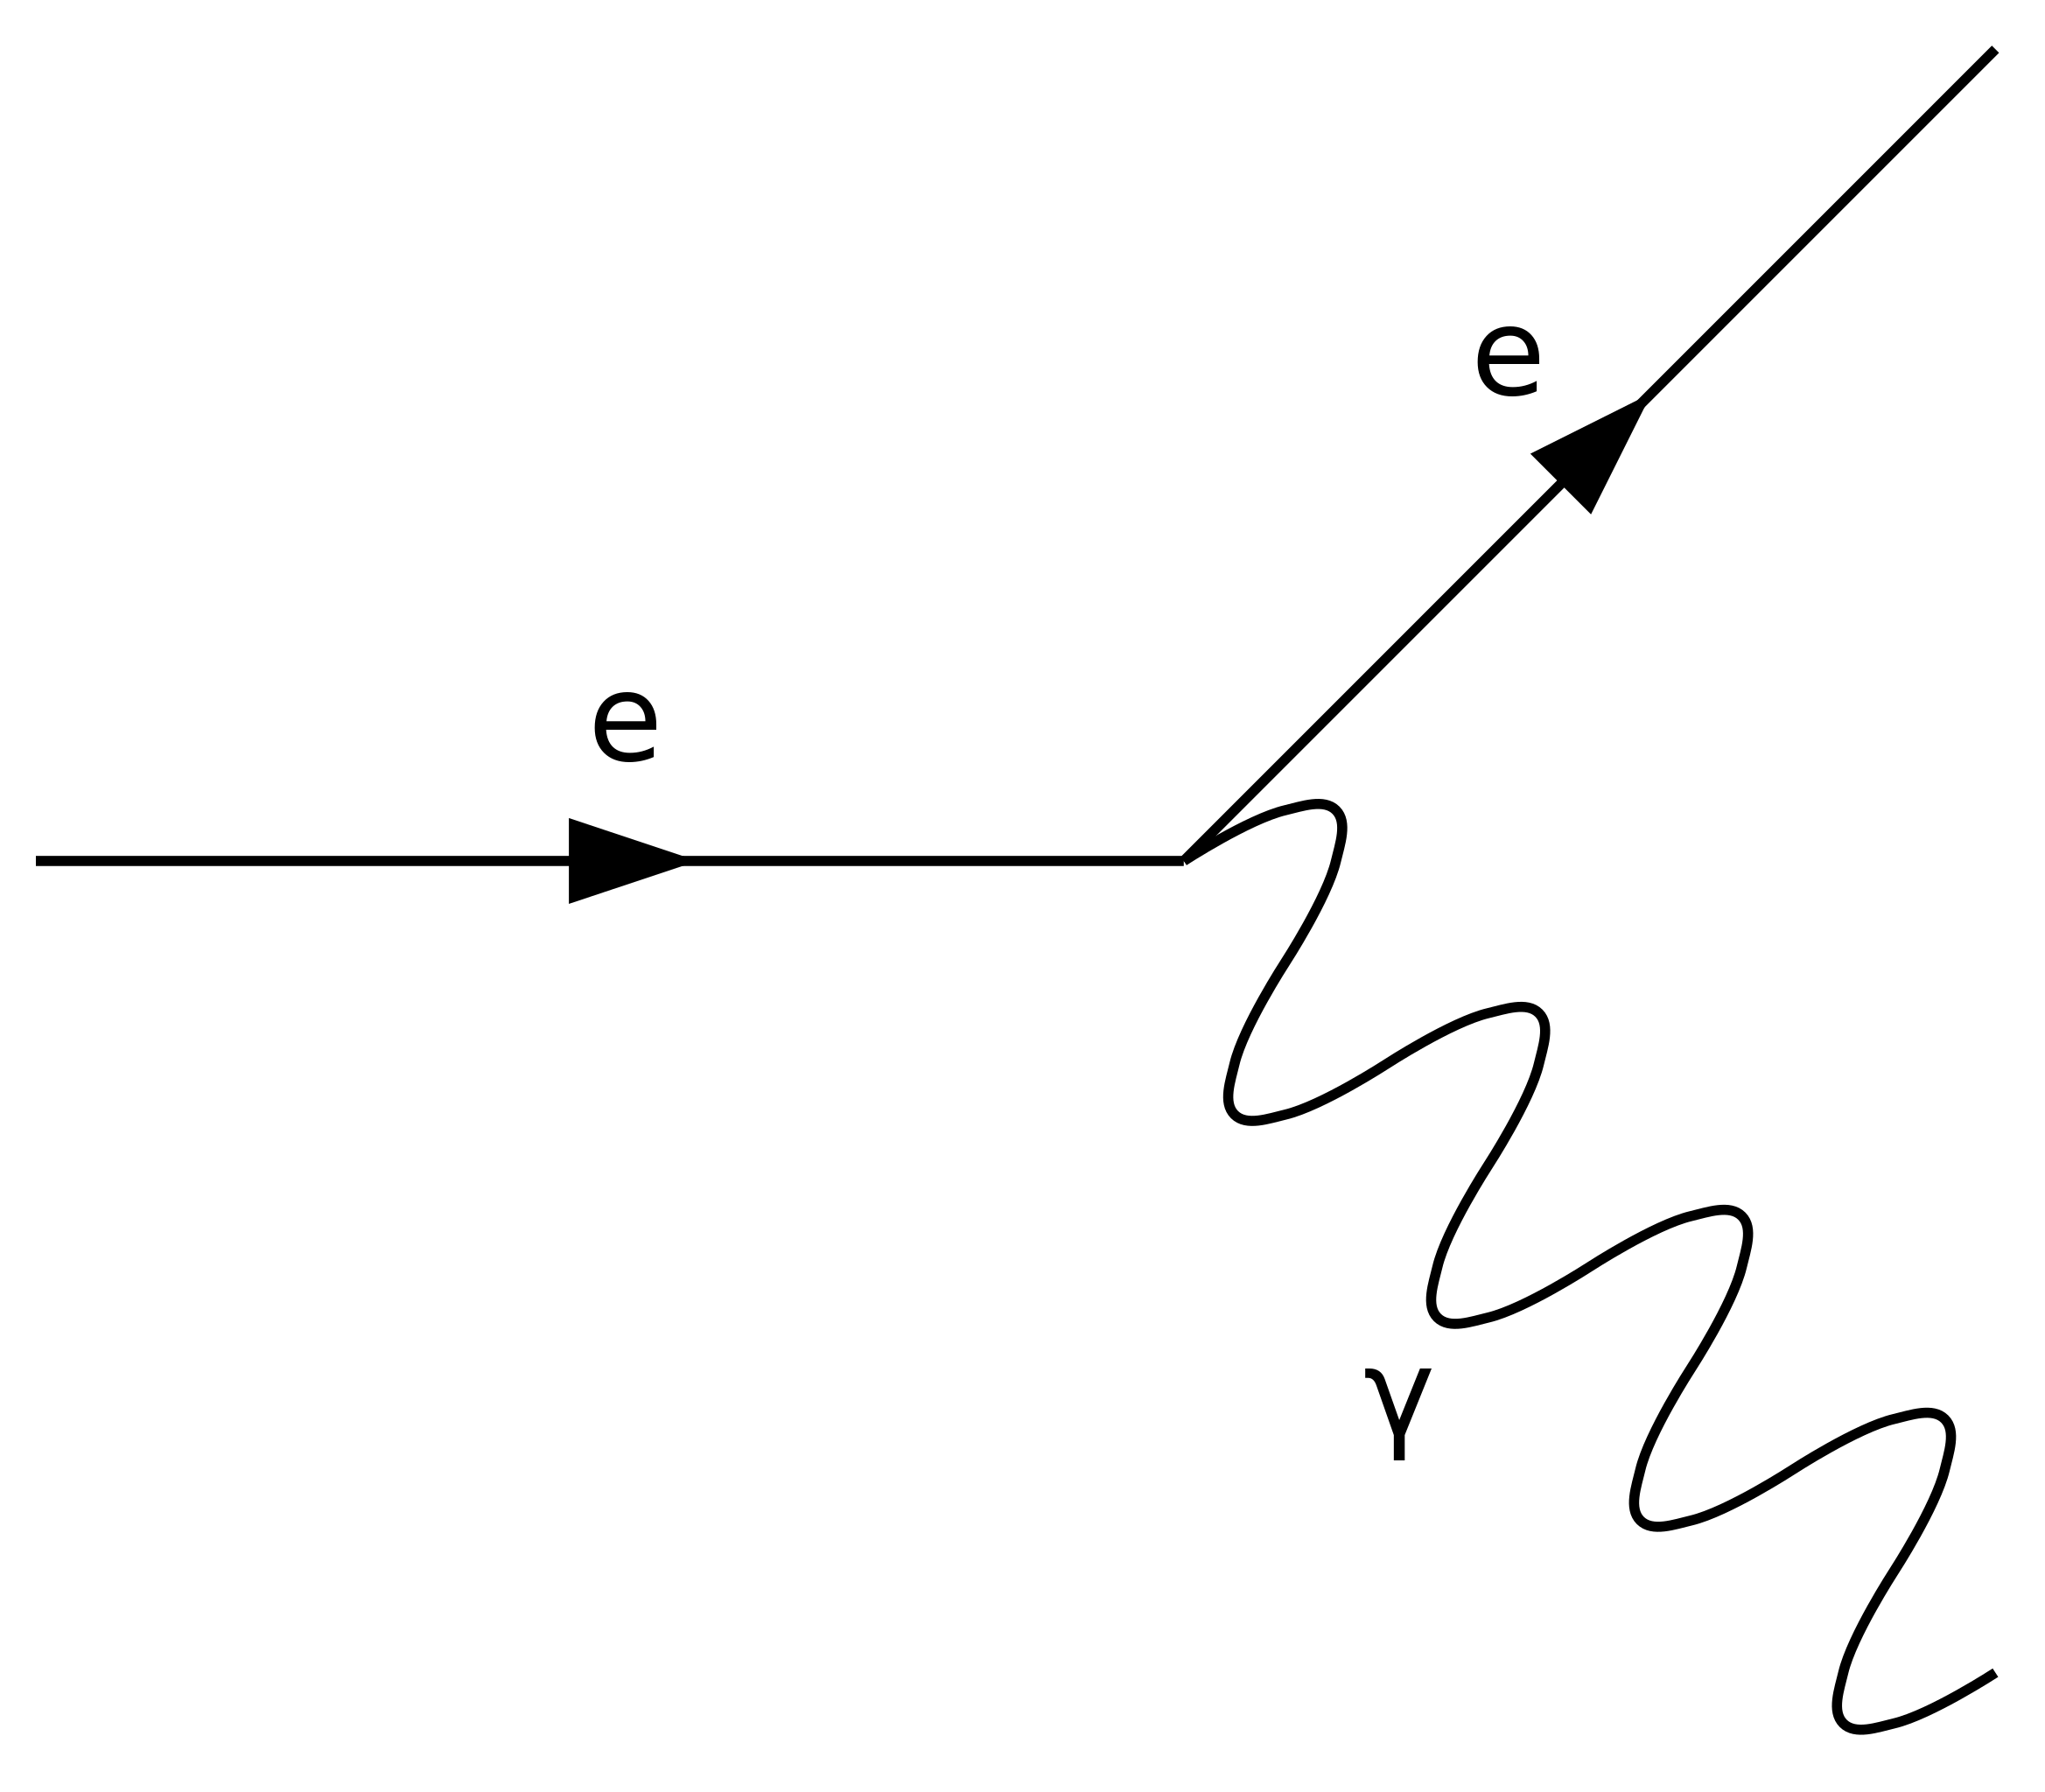
\includegraphics[width=5cm]{../Bilddateien/Feynman-electron-photon-emission.svg.png}
            \caption{Zeit von links nach rechts.}
        \end{figure}

    \subaufgabe{}
        Die Wechselwirkung zwischen zwei Elektronen $2e^{-}\stackrel{\gamma}{\longrightarrow}2e^-$ kann beschrieben werden durch das folgende Feynman-Diagramm:
        \begin{figure}[H]
            \centering
            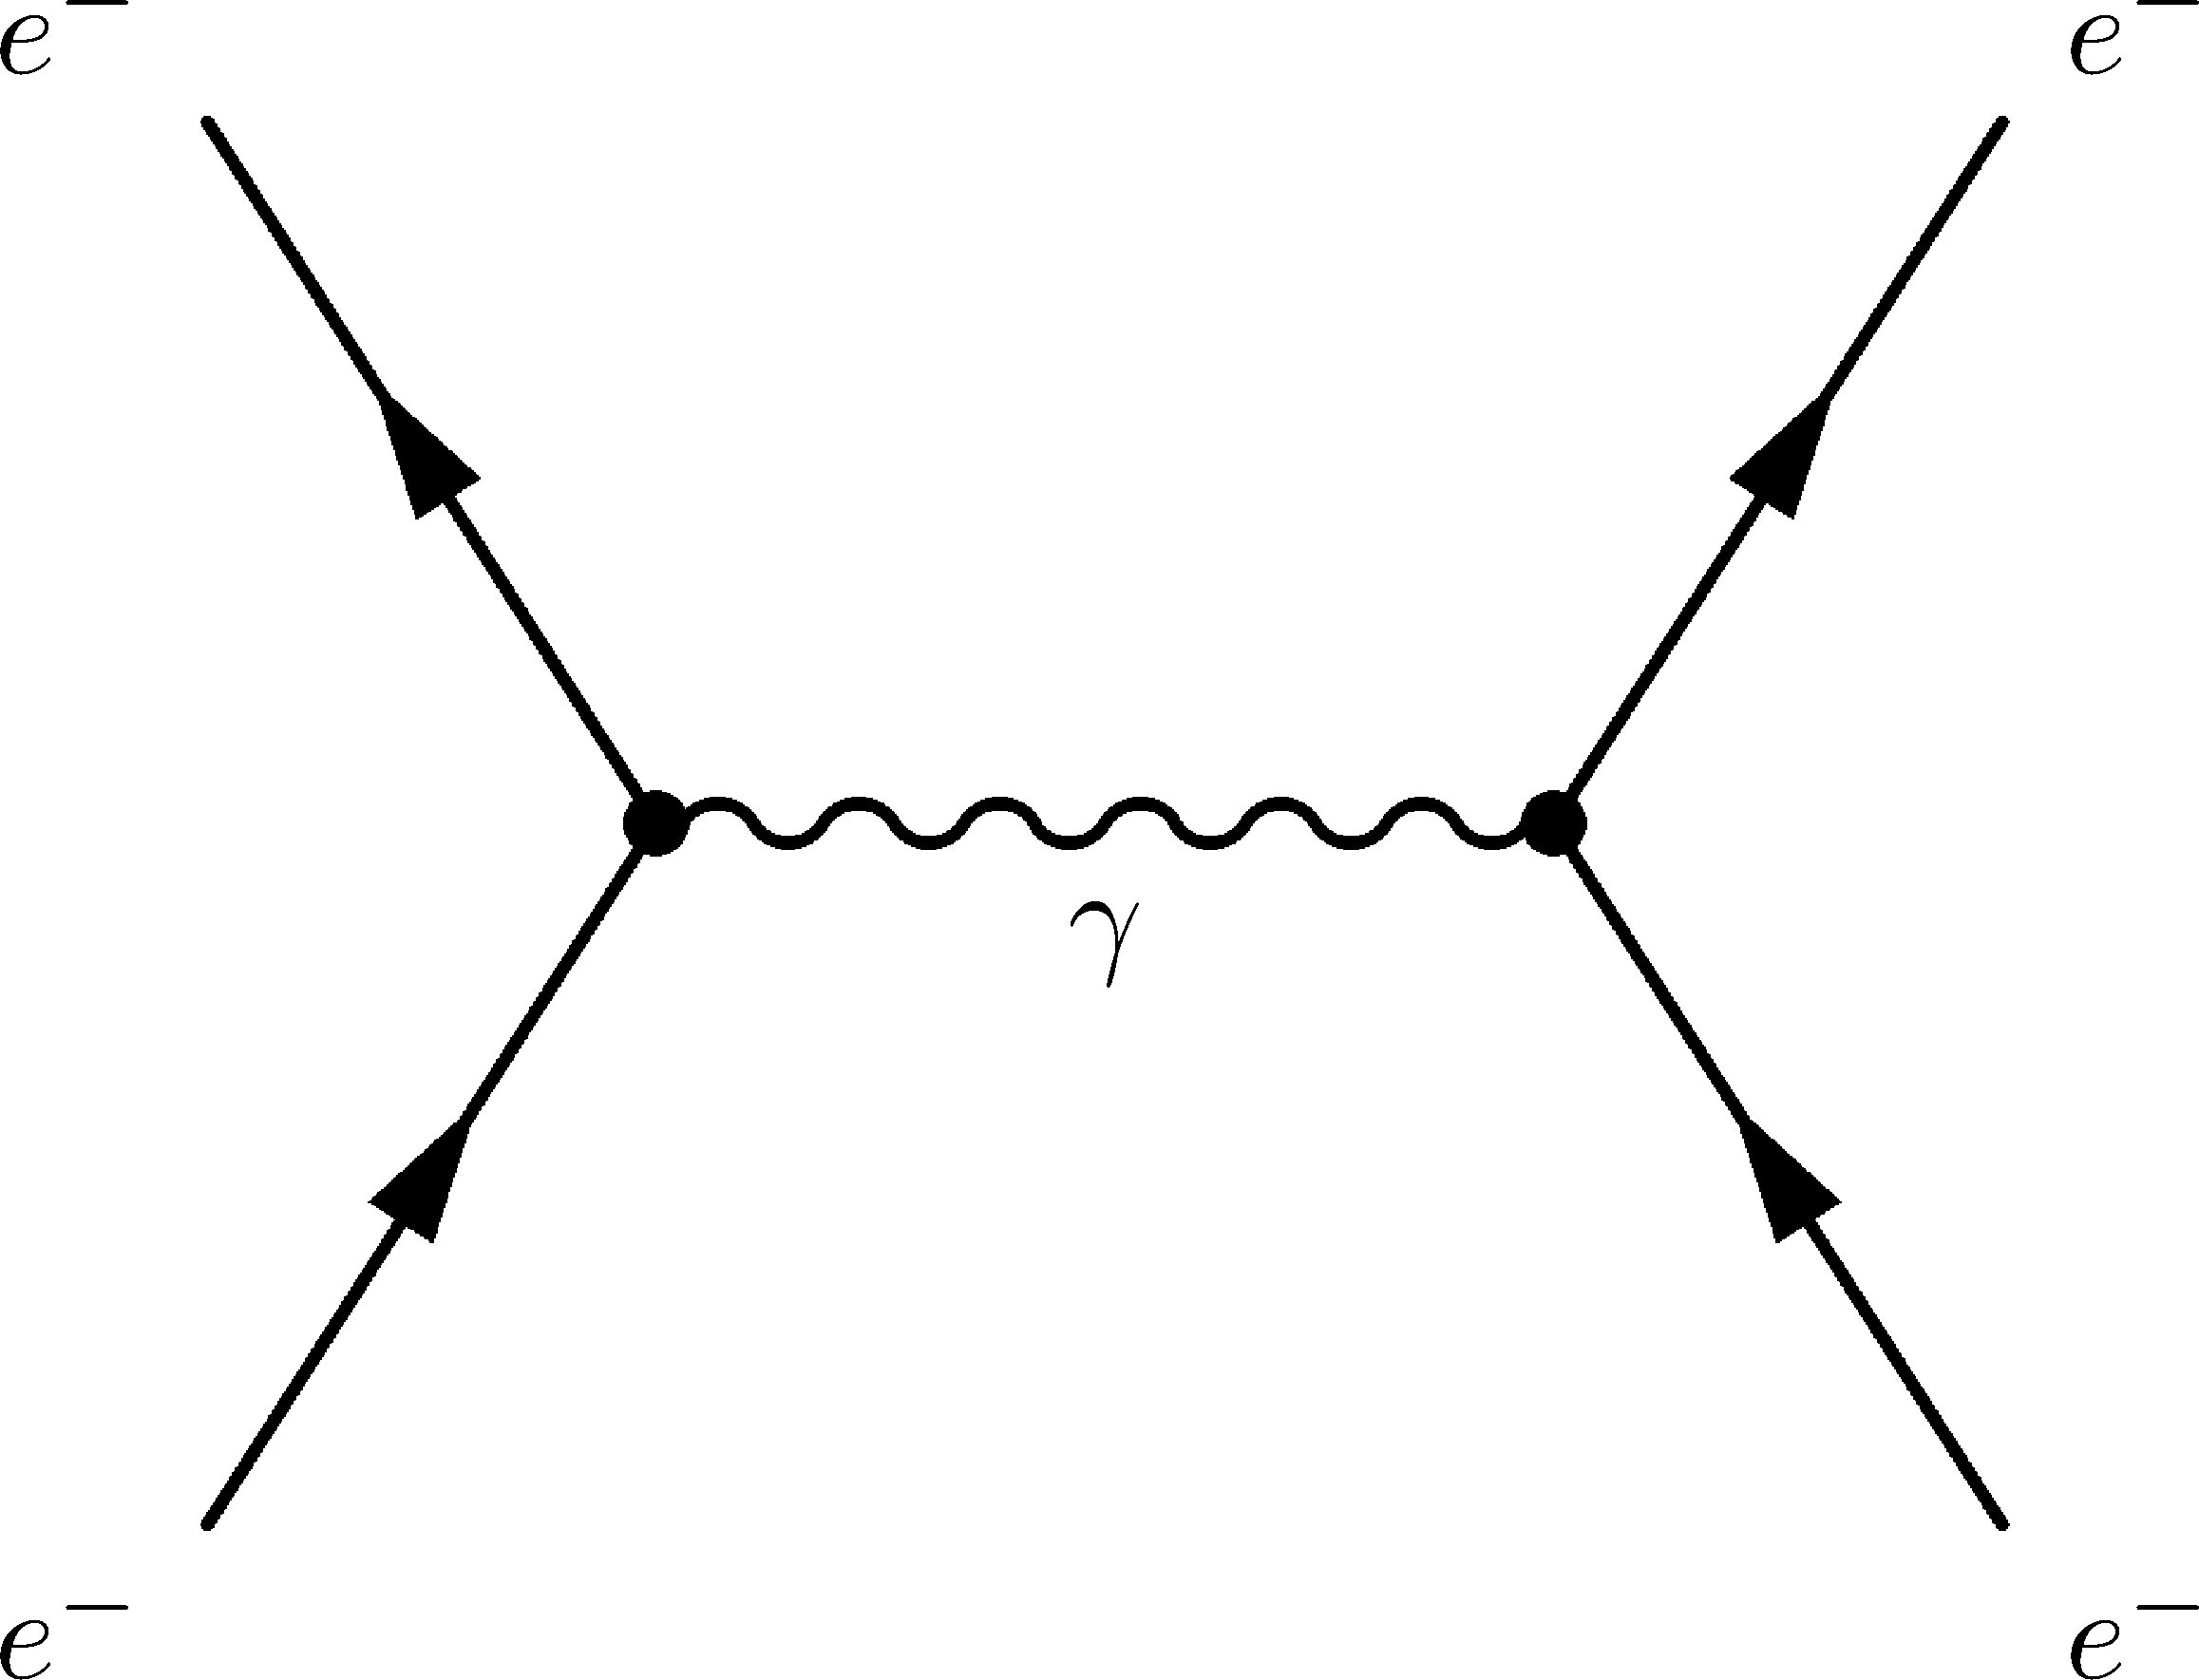
\includegraphics[width=5cm]{../Bilddateien/Feynmandiagramm.png}
            \caption{Zeit von unten nach oben.}
        \end{figure}


    \subaufgabe{}
        Die Wechselwirkung zwischen einem Elektron und einem Photon $e^{-}+\gamma\stackrel{e^-}{\longrightarrow}e^-+\gamma$ unter einem virtuellen Elektron kann beschrieben werden durch:
        \begin{figure}[H]
            \centering
            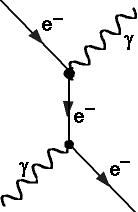
\includegraphics[height=4cm]{../Bilddateien/feyn_comp.png}
            \caption{Zeit von oben nach unten.}
        \end{figure}


    \subaufgabe{}
        Die Wechselwirkung zwischen einem Elektron und einem Photon $e^{-}+\gamma\stackrel{e^+}{\longrightarrow}e^-+\gamma$ unter einem virtuellen Positron kann beschrieben werden durch:
        \begin{figure}[H]
            \centering
            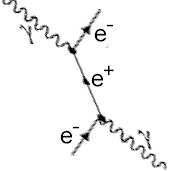
\includegraphics[height=4cm]{../Bilddateien/Unknown.png}
            \caption{Zeit von links nach rechts.}
        \end{figure}
\end{document}